%% V1.0
%% by Gabriel Garcia, gabrcg@gmail.com
%% This is a template for Udacity projects using IEEEtran.cls

%% Be Udacious!

\documentclass[10pt,journal,compsoc]{IEEEtran}

\usepackage[pdftex]{graphicx}    
\usepackage{cite}
\hyphenation{op-tical net-works semi-conduc-tor}


\begin{document}

\title{Slam Project}

\author{Jeremy Hale}

\markboth{SLAM project, Robotics Nanodegree Program, Udacity}%
{}
\IEEEtitleabstractindextext{%

\begin{abstract}
Student gives a high-level overview of what is being attempted in the report. Abstracts are typically 5-10 sentences that provide just enough context to understand the gist of the report.
\end{abstract}

% Note that keywords are not normally used for peerreview papers.
\begin{IEEEkeywords}
Robot, IEEEtran, Udacity, \LaTeX, Localization.
\end{IEEEkeywords}}


\maketitle
\IEEEdisplaynontitleabstractindextext
\IEEEpeerreviewmaketitle
\section{Introduction}
\label{sec:introduction}

\IEEEPARstart{T}{he} introduction should provide some material regarding the history of the problem, why it is important and what is intended to be achieved. If there exists any previous attempts to solve this problem, this is a great place to note these while conveying the differences in your approach (if any). The intent is to provide enough information for the reader to understand why this problem is interesting and setting up the conversation for the solution you have provided
Student can clearly and accurately explain the problem domain.

\section{Background}
Explain the importance of both mapping two and three dimensional space.

Background - The student provides a sufficient background into the scope of the problem / technologically while also identifying some of the current challenges in robot mapping and why the problem domain is an important piece of robotics. They further discuss and compare mapping algorithms

\subsection{Model Configuration}
Scene and robot configuration - Explain how your personal Gazebo world was created and what is the layout of it. Justify your choice of robot parameters, sensor location, and how you decided to configure your package structure.

Scene and robot configuration - Student explains how the gazebo world was created by providing an overview of the layout of items in his/her customized Gazebo world. Student also describes the robot's parameters, sensor features, and reasoning on the package structure.

\subsection{World Creation}
Scene and robot configuration - Explain how your personal Gazebo world was created and what is the layout of it. Justify your choice of robot parameters, sensor location, and how you decided to configure your package structure.

Scene and robot configuration - Student explains how the gazebo world was created by providing an overview of the layout of items in his/her customized Gazebo world. Student also describes the robot's parameters, sensor features, and reasoning on the package structure.

\section{Results}
Show the results of both occupancy grid and 3D map.

Results - The student should include the images for mapping process, final map (2D/3D) for both Gazebo worlds.

\begin{figure}[thpb]
    \centering
    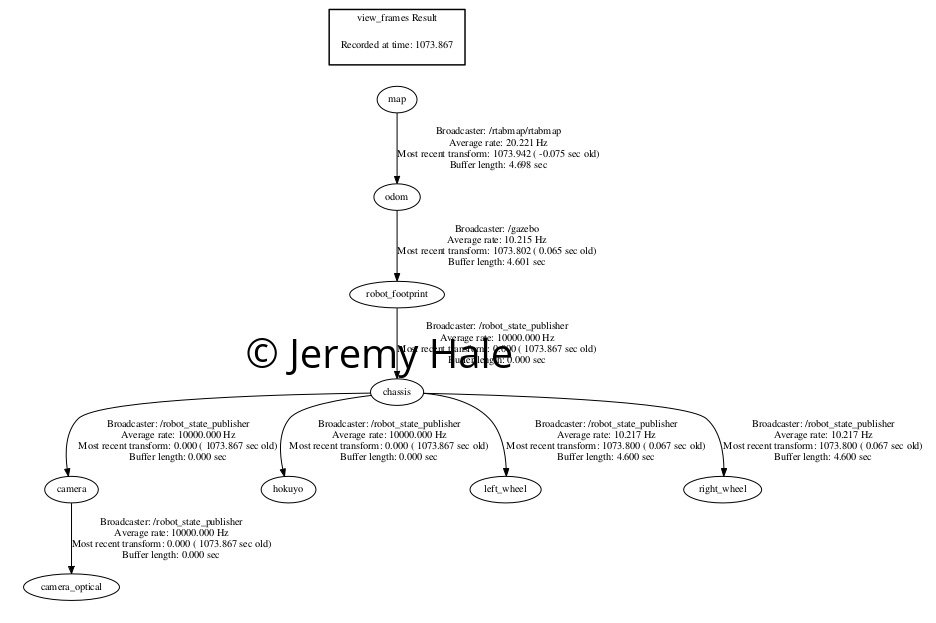
\includegraphics[width=\linewidth]{frames}
    \caption{TF Frames}
    \label{fig:frames}
\end{figure}

\begin{figure}[thpb]
    \centering
    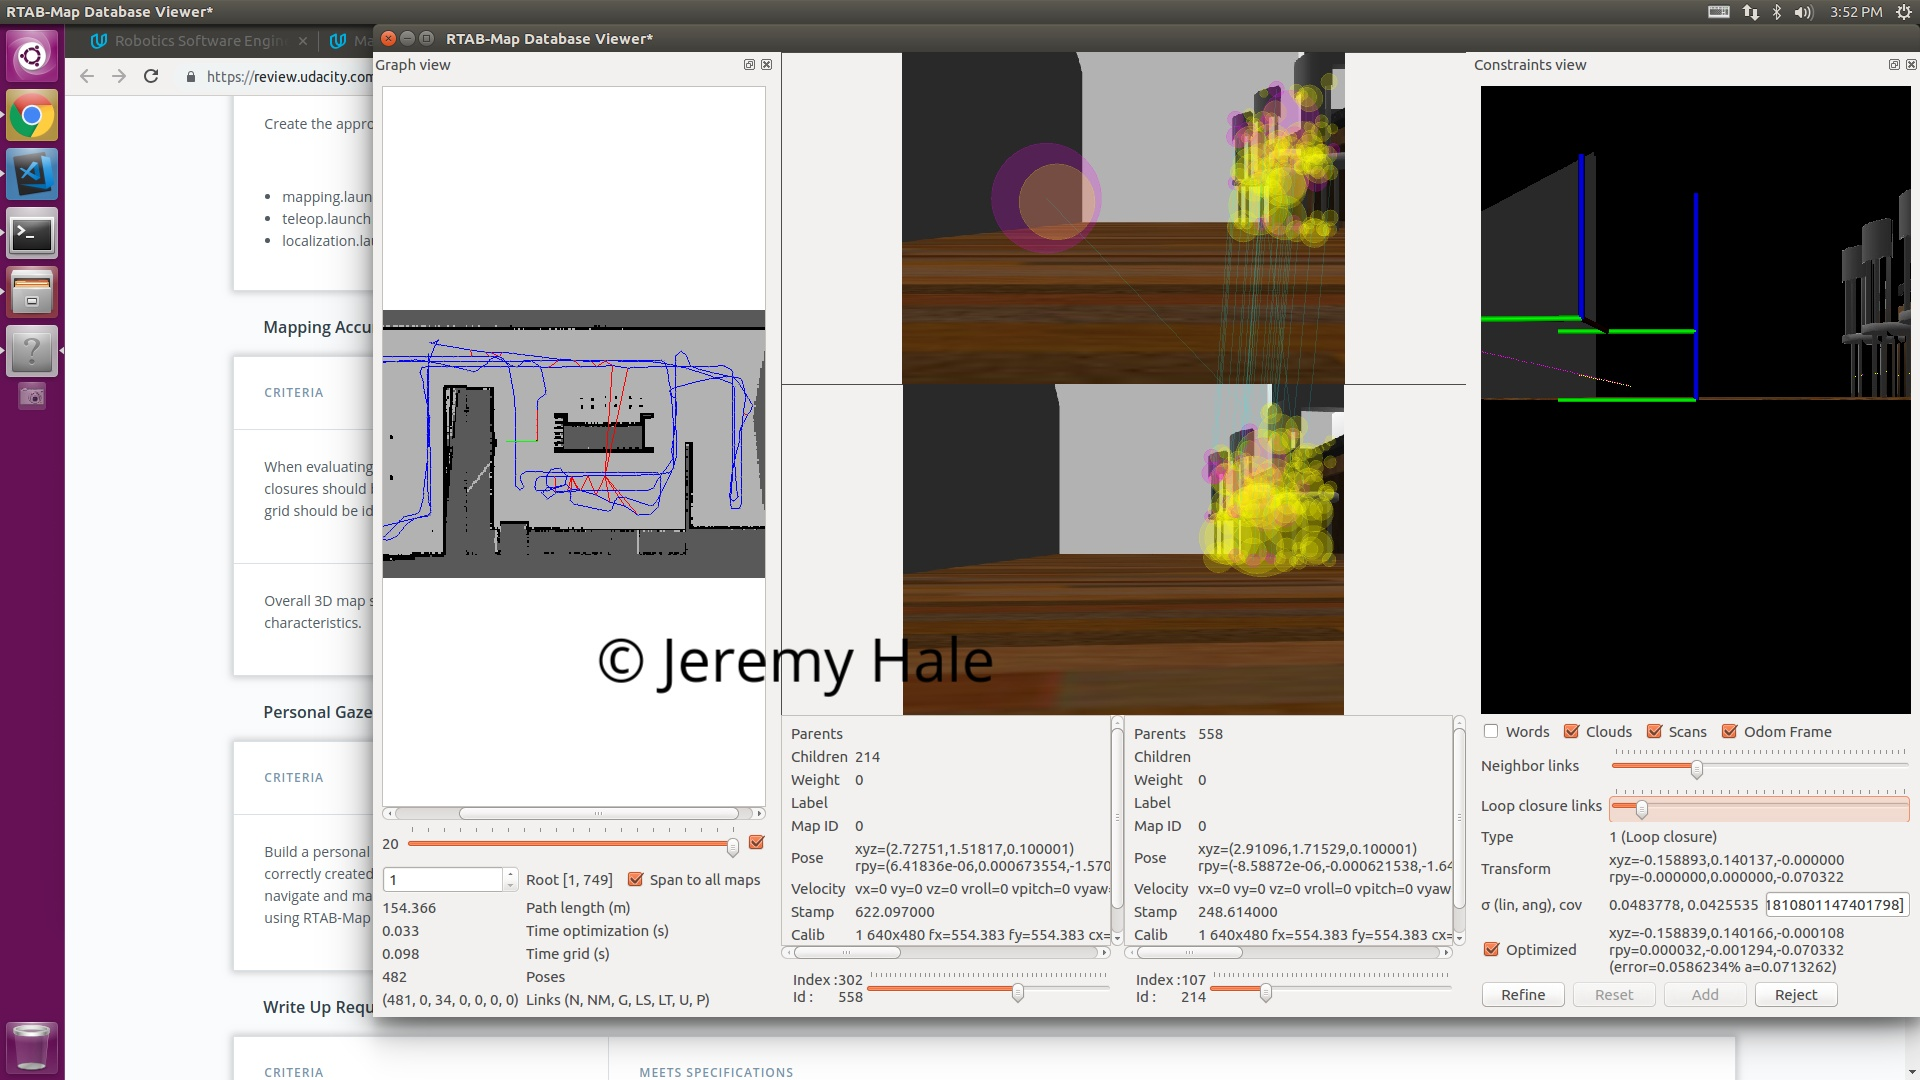
\includegraphics[width=\linewidth]{closure_1}
    \caption{Udacity World Closure}
    \label{fig:closure 1}
\end{figure}

\begin{figure}[thpb]
    \centering
    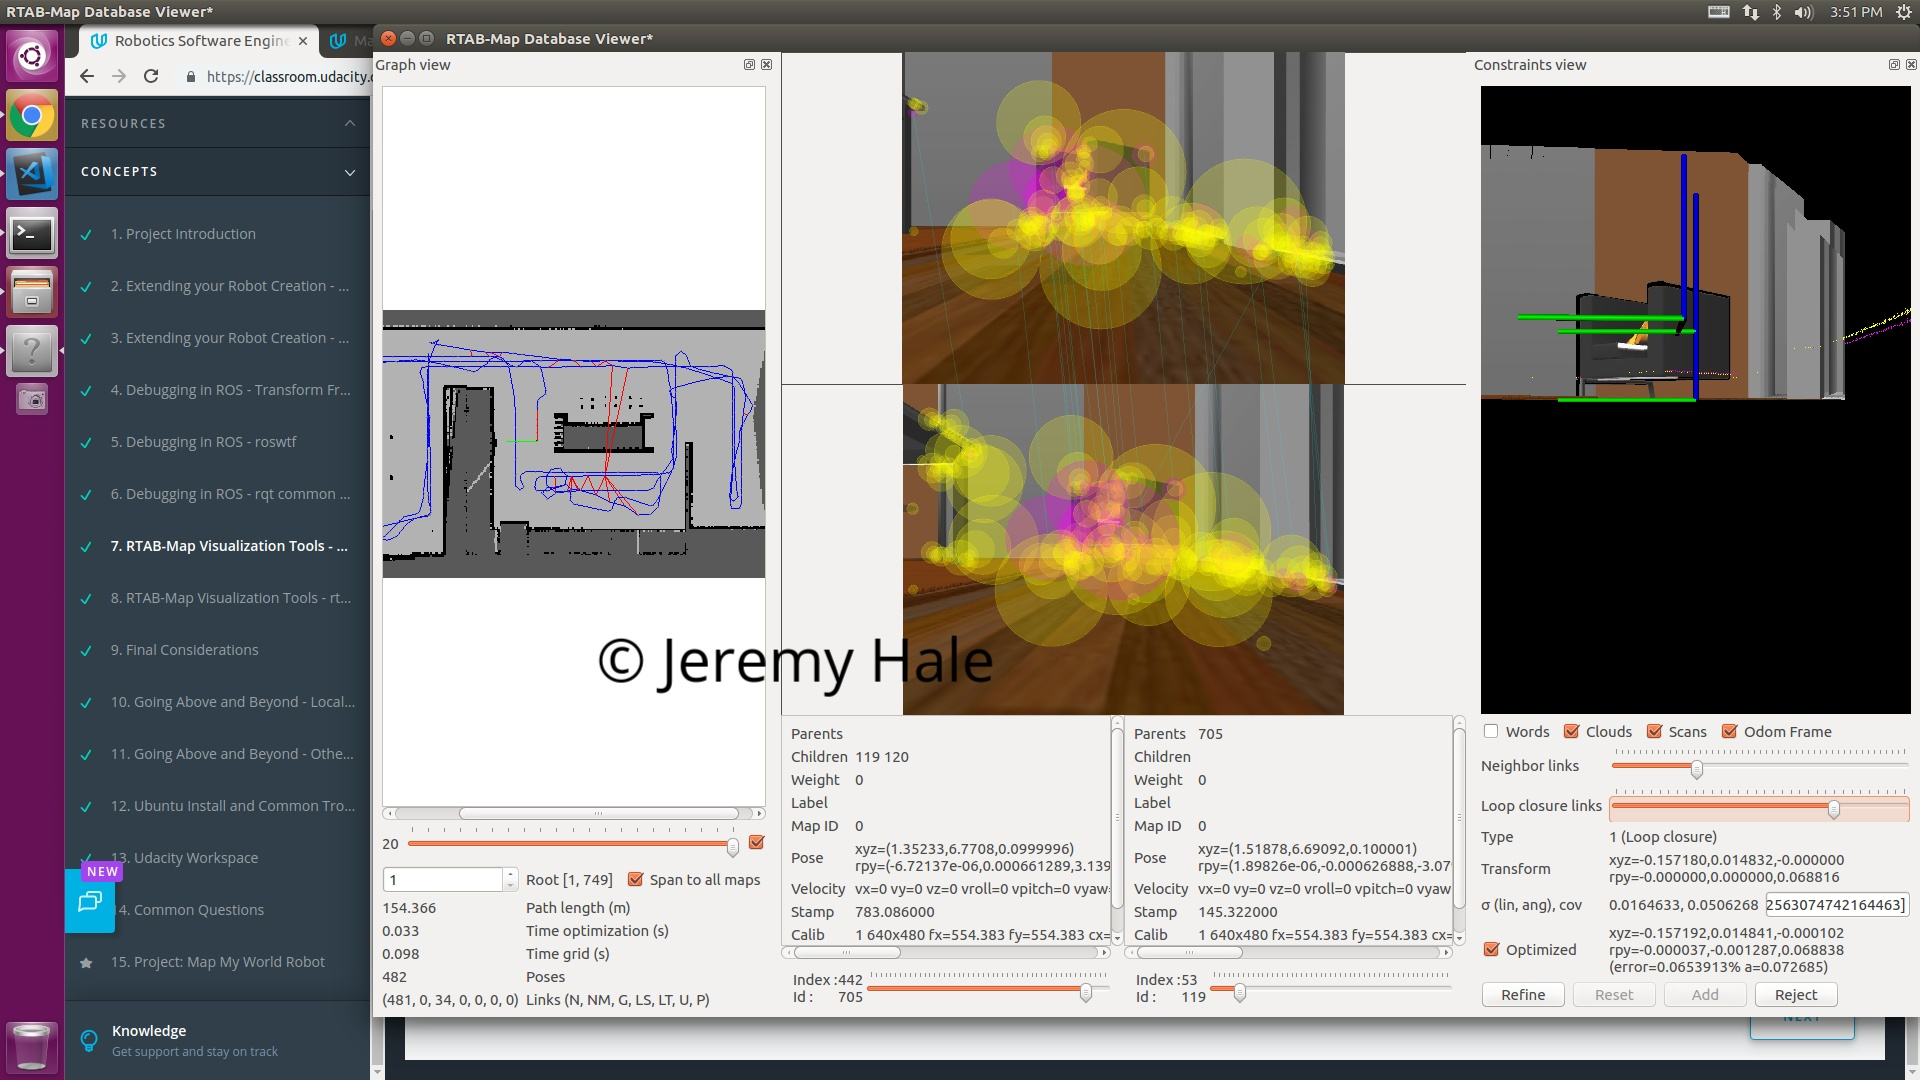
\includegraphics[width=\linewidth]{closure_2}
    \caption{Udacity World Closure}
    \label{fig:closure 2}
\end{figure}

\begin{figure}[thpb]
    \centering
    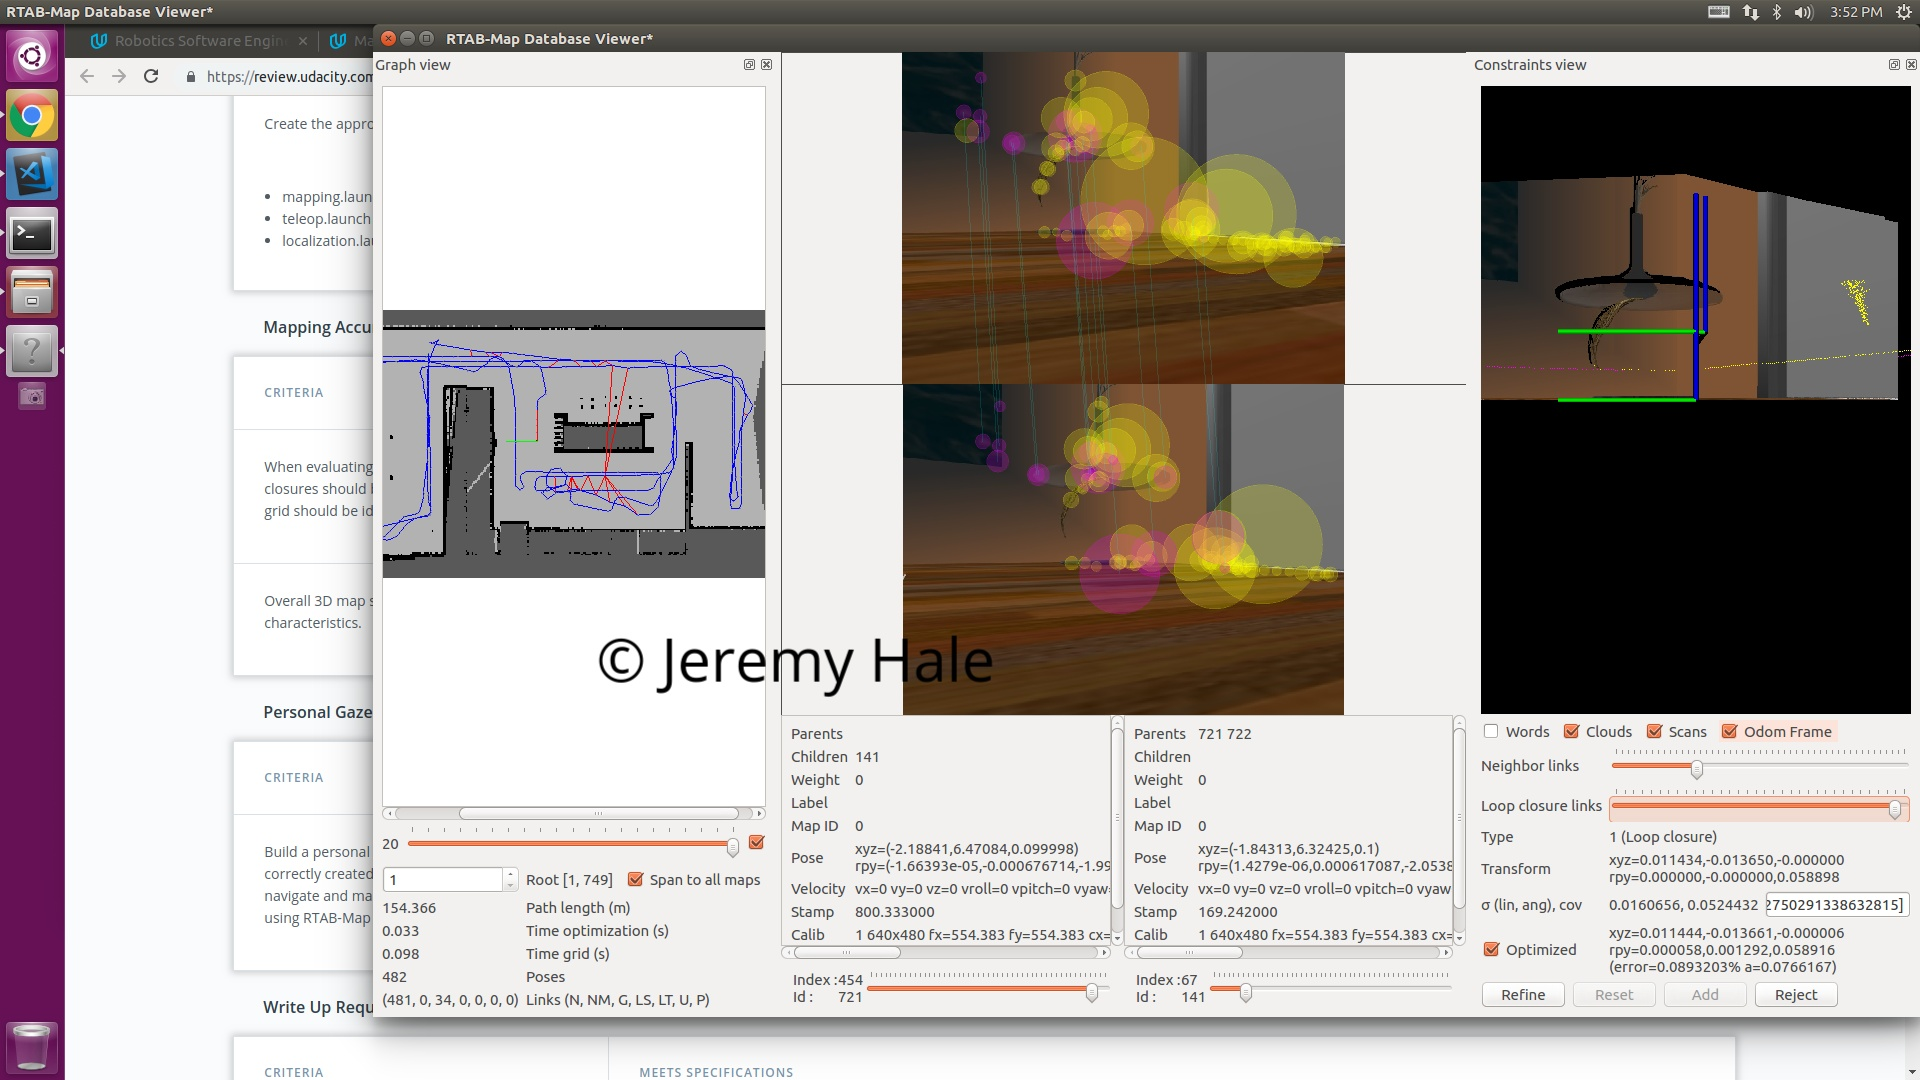
\includegraphics[width=\linewidth]{closure_3}
    \caption{Udacity World Closure}
    \label{fig:closure 3}
\end{figure}

\subsection{Localization Results}
\subsubsection{Benchmark}
\subsubsection{Student}

\section{Discussion}
What went well, what went wrong. Reflect upon the results of your robot's performance, and the performance of mapping in both worlds. Justify your answers with facts.

Discussion - The student explains how the procedure went and methodologies to improve it. The student should compare and contrast the performance of RTAB Mapping in different worlds.

\section{Conclusion / Future work}
Student discusses future desires with RTAB-Map. Talk about any robots and environment they applied this too.

"Future Work - The student can discuss how they would like to leverage this tool in robotics. The student identifies other areas where mapping could be done and for what reason. Such as simulated room or physical place.

\bibliography{bib}
\bibliographystyle{ieeetr}

\end{document}